
\pdfminorversion=4

% Modos:
% Definir el comando \handoutmode como "1" para compilar las diapositivas en
% modo handout
% al pdf generado ejecutarle el siguiente comando para poner varias diapo en una misma pagina:
%    pdfnup FILE.pdf --nup 2x3 --no-landscape --paper letterpaper --frame True
%
% Definir \handoutmode como algo distinto de "1" para compilar las diapositivas
% normalmente.
%
% Para configurar el modo desde afuera (la linea de comandos de latex) correr
% la compilacion como:
%
%   latex -output-directory=tmp -output-format=pdf '\def\handoutmode{1}\include{FILE.tex}'
%
\if\handoutmode1
    \documentclass[professionalfonts,handout]{beamer}
    \setbeameroption{show notes}
    \setbeamertemplate{note page}{\insertnote}
    \setbeamercolor{background canvas}{bg=white}
\else
    \documentclass[professionalfonts]{beamer}
\fi


% Template original the Beamer: Copyright 2004 by Till Tantau <tantau@users.sourceforge.net>.


\mode<presentation>
{
  \usetheme{metropolis}
  % or ...

  %\setbeamercovered{transparent} %hace que lo que esta covered se muestre transparente
}

\setbeamertemplate{navigation symbols}{}%remove navigation symbols

\usepackage[english]{babel}

\usepackage[latin1]{inputenc}

\usepackage{times}
\usepackage[T1]{fontenc}

% para poder escribir codigo fuente en las diapositivas
\usepackage{listings}

% para graficar diagramas simples y arboles de jerarquias
\usepackage{tikz}
\usepackage{tikz-qtree}
\usetikzlibrary{matrix,positioning}
\usetikzlibrary{shapes,arrows,chains,calc,decorations.pathmorphing}

\usepackage{xcolor}
\definecolor{darkgreen}{rgb}{0,.5,0}
\definecolor{darkblue}{rgb}{0,0,.7}
\lstdefinestyle{normal}{language=C++,       % lenguaje C++
   numbers=left,                            % enumerar las lineas
   keywordstyle=\color{darkblue}\textbf,    % color de las keywords
   stringstyle=\color{red},                 % color de los strings
   commentstyle=\color{darkgreen},          % color de los comentarios
   basicstyle=\color{black}\ttfamily\footnotesize\bfseries,     % color del texto en general
   morecomment=[l][\color{magenta}]{\#},    % coloreamos las intrucciones del precompilador (todo lo que empieza con #)
   ndkeywords={NULL,nullptr,siz,zer,mov,add},               % definimos una nuevas keywords como NULL y nullptr
   ndkeywordstyle=\color{violet},           % y las nuevas keywords tendran este color
   frame=simple,                            % simple, sin ningun marco o frame alrededor del codigo
   basewidth={0.55em,0.55em}                % tamano de las letras/lineas. usado para reducir el whitespace entre estas
}

\lstdefinestyle{normal33}{language=C++,       % lenguaje C++
   numbers=left,                            % enumerar las lineas
   keywordstyle=\color{darkblue}\textbf,    % color de las keywords
   stringstyle=\color{red},                 % color de los strings
   commentstyle=\color{darkgreen},          % color de los comentarios
   basicstyle=\color{black}\ttfamily\footnotesize\bfseries,     % color del texto en general
   morecomment=[l][\color{magenta}]{\#},    % coloreamos las intrucciones del precompilador (todo lo que empieza con #)
   ndkeywords={NULL,nullptr},               % definimos una nuevas keywords como NULL y nullptr
   ndkeywordstyle=\color{violet},           % y las nuevas keywords tendran este color
   frame=simple,                            % simple, sin ningun marco o frame alrededor del codigo
   basewidth={0.55em,0.55em}                % tamano de las letras/lineas. usado para reducir el whitespace entre estas
}
%mismo estilo, sin numeros
\lstdefinestyle{normalnonumbers}{language=C++,
   keywordstyle=\color{darkblue}\textbf,
   stringstyle=\color{red},           
   commentstyle=\color{darkgreen},    
   basicstyle=\color{black}\ttfamily\footnotesize\bfseries,
   morecomment=[l][\color{magenta}]{\#},
   ndkeywords={NULL,nullptr,move,add},          
   ndkeywordstyle=\color{violet}, 
   frame=simple,
   basewidth={0.55em,0.55em}
}


% mismo estilo pero todos los colores estan mas debiles como si se volvieran transparentes
% usado para poder resaltar el codigo.
\lstdefinestyle{dimmided}{language=C++,
   keywordstyle=\color{darkblue!30}\textbf,
   stringstyle=\color{red!30},
   commentstyle=\color{darkgreen!30},
   basicstyle=\color{black!30}\ttfamily\footnotesize\bfseries,
   morecomment=[l][\color{magenta!30}]{\#},
   ndkeywords={NULL,nullptr,siz,zer,mov,add},
   ndkeywordstyle=\color{violet!30}, 
   moredelim=**[is][\only<+->{\color{black}\lstset{style=normal}}]{@}{@}, % definimos que las lineas entre arrobas (@) tendran el estilo normal (con los colores a toda intensidad)
   frame=simple,
   basewidth={0.55em,0.55em}
}
\lstdefinestyle{dimmided42}{language=C++,
   keywordstyle=\color{darkblue!30}\textbf,
   stringstyle=\color{red!30},
   commentstyle=\color{darkgreen!30},
   basicstyle=\color{black!30}\ttfamily\footnotesize\bfseries,
   morecomment=[l][\color{magenta!30}]{\#},
   ndkeywords={NULL,nullptr,siz,zer,mov,add},
   ndkeywordstyle=\color{violet!30}, 
   moredelim=**[is][{\color{black}\lstset{style=normal}}]{@}{@}, % definimos que las lineas entre arrobas (@) tendran el estilo normal (con los colores a toda intensidad)
   frame=simple,
   basewidth={0.55em,0.55em}
}

\lstdefinelanguage{json}{
    literate=
     *{:}{{{\color{violet}{:}}}}{1}
      {,}{{{\color{violet}{,}}}}{1}
      {\{}{{{\color{darkgreen}{\{}}}}{1}
      {\}}{{{\color{darkgreen}{\}}}}}{1}
      {[}{{{\color{darkgreen}{[}}}}{1}
      {]}{{{\color{darkgreen}{]}}}}{1},
}


\lstdefinestyle{normaljson}{language=json,  % lenguaje json
   numbers=left,                            % enumerar las lineas
   keywordstyle=\color{darkblue}\textbf,    % color de las keywords
   stringstyle=\color{red},                 % color de los strings
   commentstyle=\color{red},                % color de los comentarios
   basicstyle=\color{black}\ttfamily\footnotesize\bfseries,     % color del texto en general
   morecomment=[l][\color{magenta}]{\#},    % coloreamos las intrucciones del precompilador (todo lo que empieza con #)
   ndkeywords={NULL,nullptr},               % definimos una nuevas keywords como NULL y nullptr
   ndkeywordstyle=\color{violet},           % y las nuevas keywords tendran este color
   frame=simple,                            % simple, sin ningun marco o frame alrededor del codigo
   basewidth={0.55em,0.55em}                % tamano de las letras/lineas. usado para reducir el whitespace entre estas
}

\lstdefinelanguage{http}{
    morekeywords={
        GET,
        PUT,
        POST,
        DELETE
    }
}

\lstdefinestyle{normalhttp}{language=http,  % lenguaje HTTP
   numbers=left,                            % enumerar las lineas
   keywordstyle=\color{darkblue}\textbf,    % color de las keywords
   stringstyle=\color{red},                 % color de los strings
   commentstyle=\color{red},                % color de los comentarios
   basicstyle=\color{black}\ttfamily\footnotesize\bfseries,     % color del texto en general
   morecomment=[l][\color{magenta}]{\#},    % coloreamos las intrucciones del precompilador (todo lo que empieza con #)
   ndkeywords={NULL,nullptr},               % definimos una nuevas keywords como NULL y nullptr
   ndkeywordstyle=\color{violet},           % y las nuevas keywords tendran este color
   frame=simple,                            % simple, sin ningun marco o frame alrededor del codigo
   basewidth={0.55em,0.55em}                % tamano de las letras/lineas. usado para reducir el whitespace entre estas
}

% Pone las constantes numericas con color (violeta en este caso):
% - los numeros que estan dentro de un string/comentarios NO son coloreados
% - los numeros por fuera que pertenecen a una palabra SON coloreados 
%   (buf1, por ejemplo, el "1" es coloreado cuando no lo deberias. UPS!!)
% - No incluye el signo
% 
%\lstset{literate=%
%  *{0}{{{\color{violet}0}}}1
%   {1}{{{\color{violet}1}}}1
%   {2}{{{\color{violet}2}}}1
%   {3}{{{\color{violet}3}}}1
%   {4}{{{\color{violet}4}}}1
%   {5}{{{\color{violet}5}}}1
%   {6}{{{\color{violet}6}}}1
%   {7}{{{\color{violet}7}}}1
%   {8}{{{\color{violet}8}}}1
%   {9}{{{\color{violet}9}}}1
%}

% Para resaltar lineas de codigo usando \btLstHLB{range} y \btLstHLB<overlay>{range}:
% Por ejemplo, 
%  \btLstHLB{3}       linea 3 resaltada
%  \btLstHLB{1-5}     lineas de la 1 a la 5 resaltadas
%  \btLstHLB<2>{3}    linea 3 resaltada solo en el slide 2
%
% \btLstHLB usa un color azul mientras que \btLstHLR usa un color rojo como fondo
\usepackage{lstlinebgrd}
\makeatletter
\newcount\bt@rangea
\newcount\bt@rangeb

\newcommand\btIfInRange[2]{%
   \global\let\bt@inrange\@secondoftwo%
   \edef\bt@rangelist{#2}%
   \foreach \range in \bt@rangelist {%
      \afterassignment\bt@getrangeb%
      \bt@rangea=0\range\relax%
      \pgfmathtruncatemacro\result{ ( #1 >= \bt@rangea) && (#1 <= \bt@rangeb) }%
      \ifnum\result=1\relax%
      \breakforeach%
      \global\let\bt@inrange\@firstoftwo%
      \fi%
   }%
   \bt@inrange%
}
\newcommand\bt@getrangeb{%
   \@ifnextchar\relax%
   {\bt@rangeb=\bt@rangea}%
   {\@getrangeb}%
}
\def\@getrangeb-#1\relax{%
   \ifx\relax#1\relax%
      \bt@rangeb=100000%   \maxdimen is too large for pgfmath
   \else%
      \bt@rangeb=#1\relax%
   \fi%
}

%%%%%%%%%%%%%%%%%%%%%%%%%%%%%%%%%%%%%%%%%%%%%%%%%%%%%%%%%%%%%%%%%%%%%%%%%%%%%%
%
% \btLstHL<overlay spec>{range list}
%
\newcommand<>{\btLstHLB}[1]{%
   \only#2{\btIfInRange{\value{lstnumber}}{#1}{\color{blue!30}}% blue
   {\def\lst@linebgrdcmd####1####2####3{}}}%
}%
\newcommand<>{\btLstHLR}[1]{%
   \only#2{\btIfInRange{\value{lstnumber}}{#1}{\color{red!30}}% red
   {\def\lst@linebgrdcmd####1####2####3{}}}%
}%
%
%
%%%%%%%%%%%%%%%%%%%%%%

\makeatother


% sin fecha
\date{}

\author[7542]{Di Paola Mart\'in \\ \texttt{martinp.dipaola <at> gmail.com} }

\institute[Universidad de Buenos Aires]
{
   Facultad de Ingenier\'ia\\
   Universidad de Buenos Aires
}

% Definimos una imagen para que este en cada slide
%\pgfdeclareimage[height=0.5cm]{university-logo}{imgs/fiuba.png}
%\logo{\pgfuseimage{university-logo}}

%% Definir estas en el documento final
%%
%% \title%
%% {Programaci\'on gen\'erica y templates en C++}
%%
%% \subject{Programaci\'on gen\'erica y templates en C++}


%%%%%
% At begin of each Section do nothing; at each Subsection show the Section and Subsection names
% If the Section doesn't have a Subsection, then YOU must to add a unnumbered Subsection like \subsection*{}
% so the AtBeginSubsection will get triggered
\AtBeginSection{}
\AtBeginSubsection[\frame{\subsectionpage}]{\frame{\subsectionpage}}
%
%%%%%




\title%
{Herencia y Polimorfismo}

\subject{Herencia y Polimorfismo}

\begin{document}

\begin{frame}
   \titlepage
\end{frame}

\begin{frame}{Contenidos}
   \tableofcontents
   % You might wish to add the option [pausesections]
\end{frame}

\section{Herencia}
\subsection{\textquestiondown Qu\'e es la Herencia?}
\begin{frame}[plain,fragile]{Herencia}{}
   \begin{enumerate}
      \item Es un concepto de la OOP
      \item Establece una relaci\'on \textbf{"es un"}
      \item Se dice que:
      \begin{enumerate}
         \item Una clase \textit{derivada} \textbf{extiende} a una clase \textit{base}.
         \item Una clase \textit{base} \textbf{generaliza} varias clases \textit{derivadas}.
      \end{enumerate}
   \end{enumerate}

   \begin{figure}
      \centering

      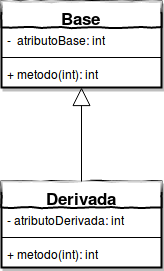
\includegraphics[height=0.5\textheight]{./Herencia.png}
   \end{figure}
\end{frame}

\subsection{Herencia en C++}

\begin{frame}[plain,fragile]{Herencia en C++}{
En C++ heredamos indicando un tipo de herencia (usaremos public por default)\newline
   }
   \begin{lstlisting}[style=normal,firstnumber=1,linebackgroundcolor={%
           \btLstHLB<1>{5}%
   }]
class Base {
  ...
};

class Derivada: public Base {
  ...
};

   \end{lstlisting}
   \begin{enumerate}
      \item No se heredan:
      \begin{enumerate}
         \item Los constructores
         \item Los operadores
         \item friend
      \end{enumerate}
      \item Tambi\'en se puede heredar en forma protected o private.
   \end{enumerate}

\end{frame}

\begin{frame}[plain,fragile]{\textquestiondown C\'omo llamamos al constructor de Base?}{
  \textexclamdown No podemos acceder a los miembros private de la clase base!
}
   \begin{lstlisting}[style=normal,firstnumber=1]
class Base {
private:
  int entero;

public:
  Base(int entero): entero(entero) {
  }
};

class Derivada: public Base {
public:
  Derivada(int entero): Base(entero) {
  }
};

   \end{lstlisting}
   \begin{enumerate}
      \item Para delegar el constructor usamos la \textbf{member initializer list}.
      \item En C++ el constructor de Base se llama antes que el constructor de Derivada.
      \item Con los destructores es al rev\'es (como una pila).
   \end{enumerate}

\end{frame}

\section{Polimorfismo}
\subsection{\textquestiondown Qu\'e es el Polimorfismo?}
\begin{frame}[plain,fragile]{Polimorfismo}{}
   \begin{enumerate}
      \item Tener varias formas.
      \item En C++, significa que la misma llamada a funci\'on tiene distintos comportamientos dependiendo del tipo del \textbf{objeto}.
      \item No queremos que dependa del tipo de la \textbf{variable}.
   \end{enumerate}
\end{frame}

\subsection{Polimorfismo en C++}
\begin{frame}[plain,fragile]{Polimorfismo en C++}{
\textquestiondown Cu\'al es la salida de este c\'odigo?
}
   \begin{columns}[t]
      \begin{column}{.6\linewidth}
         \begin{lstlisting}[style=normal,firstnumber=1]
#include <iostream>

class Base {
public:
  void metodo() {
    std::cout << "Base\n";
  }
};

class Derivada1: public Base {
public:
  void metodo() {
    std::cout << "Derivada 1\n";
  }
};

class Derivada2: public Base {
public:
  void metodo() {
    std::cout << "Derivada 2\n";
  }
};

         \end{lstlisting}
      \end{column}
      \begin{column}{.4\linewidth}
         \begin{lstlisting}[style=normal,firstnumber=25]
int main(void) {
  Base *ptr;
  Derivada1 d1;
  Derivada2 d2;

  ptr = &d1;
  ptr->metodo();

  ptr = &d2;
  ptr->metodo();

  return 0;
}
         \end{lstlisting}

      La salida ser\'a:\newline \texttt{Base\newline Base\newline}
      \end{column}
   \end{columns}
\end{frame}
\note[itemize] {
   \item Por defecto, C++ resuelve a qu\'e m\'etodo llamar en tiempo de compilaci\'on.
   \item A esto se lo conoce como \textbf{static linkage, static resolution, o early binding}.
   \item Para que esto se resuelva en tiempo de ejecuci\'on debemos usar el modificador \textbf{virtual}.
   \item En Java todo es virtual por defecto, y para que no sea virtual hay que usar \textbf{final}.
   \item Usar virtual crea \textbf{VTable}s, que sirven para la resoluci\'on din\'amica, lo cual empeora la performance.
   \item A esto se lo conoce como \textbf{dynamic linkage, o late binding}.
}

\begin{frame}[plain,fragile]{Polimorfismo en C++}{
Usando el modificador \textbf{virtual}.
}
   \begin{columns}[t]
      \begin{column}{.6\linewidth}
         \begin{lstlisting}[style=normal,firstnumber=1]
#include <iostream>

class Base {
public:
  virtual void metodo() {
    std::cout << "Base\n";
  }
};

class Derivada1: public Base {
public:
  virtual void metodo() {
    std::cout << "Derivada 1\n";
  }
};

class Derivada2: public Base {
public:
  virtual void metodo() override {
    std::cout << "Derivada 2\n";
  }
};

         \end{lstlisting}
      \end{column}
      \begin{column}{.4\linewidth}
         \begin{lstlisting}[style=normal,firstnumber=25]
int main(void) {
  Base *ptr;
  Derivada1 d1;
  Derivada2 d2;

  ptr = &d1;
  ptr->metodo();

  ptr = &d2;
  ptr->metodo();

  return 0;
}
         \end{lstlisting}

      La salida ser\'a:\newline \texttt{Derivada 1\newline Derivada 2\newline}
      \end{column}
   \end{columns}
\end{frame}
\note[itemize] {
   \item Notar que la variable \textbf{ptr} siempre es de tipo \textbf{Base*}, lo que cambia es el tipo del \textbf{objeto}.
   \item Esto nos permite, por ejemplo, tener una lista de punteros a \textbf{Base}, e iterarla llamando siempre a \textbf{metodo()}, sin depender del tipo del objeto en tiempo de compilaci\'on.
   \item El identificador \textbf{override} (C++11) obliga a que la firma coincida con la del m\'etodo de la clase base.
}

\begin{frame}[plain,fragile]{\textquestiondown C\'omo llamamos un m\'etodo de Base desde Derivada?}
   \begin{columns}[t]
      \begin{column}{.6\linewidth}
         \begin{lstlisting}[style=normal,firstnumber=1]
#include <iostream>

class Base {
public:
  virtual void metodo() {
    std::cout << "Base\n";
  }
};

class Derivada: public Base {
public:
  virtual void metodo() {
    std::cout << "Derivada\n";
    Base::metodo();
  }
};

         \end{lstlisting}
      \end{column}
      \begin{column}{.4\linewidth}
         \begin{lstlisting}[style=normal,firstnumber=25]
int main(void) {
  Derivada d;
  d.metodo();

  return 0;
}
         \end{lstlisting}

      La salida ser\'a:\newline \texttt{Derivada\newline Base\newline}
      \end{column}
   \end{columns}
\end{frame}

\subsection{Clases abstractas e Interfaces}
\begin{frame}[plain,fragile]{Clases abstractas}{
Las clases abstractas son las que tienen un \textbf{m\'etodo virtual puro}.
}

   \begin{columns}[t]
      \begin{column}{.6\linewidth}
         \begin{lstlisting}[style=normal,firstnumber=1]
#include <iostream>

class Base {
public:
  virtual void metodo() = 0;
};

class Derivada1: public Base {
public:
  virtual void metodo() {
    std::cout << "Derivada 1\n";
  }
};

class Derivada2: public Base {
public:
  virtual void metodo() {
    std::cout << "Derivada 2\n";
  }
};

         \end{lstlisting}
      \end{column}
      \begin{column}{.4\linewidth}
         \begin{lstlisting}[style=normal,firstnumber=23,linebackgroundcolor={%
                 \btLstHLR<1>{24,25}%
         }]
int main(void) {
  // no compila!
  Base base; 
  Derivada1 d1;
  Derivada2 d2;

  return 0;
}
         \end{lstlisting}

      \end{column}
   \end{columns}
\end{frame}
\note[itemize] {
   \item No se puede instanciar una clase abstracta.
   \item En C++ no existe un modificador \textit{abstract}, una clase abstracta es la que tiene un m\'etodo virtual puro.
   \item La \'unica manera de hacer interfaces en C++ es usando clases abstractas sin atributos.
}

\subsection{Destructores virtuales}
\begin{frame}[plain,fragile]{Destructores virtuales}{}
   \begin{columns}[t]
      \begin{column}{.5\linewidth}
         \begin{lstlisting}[style=normal,firstnumber=1]
class Base {
public:
  Base() {
    std::cout << "Base\n";
  }

  ~Base() {
    std::cout << "Destr Base\n";
  }
};

class Derivada: public Base {
public:
  Derivada() {
    std::cout << "Derivada\n";
  }

  ~Derivada() {
    std::cout << "Destr Derivada\n";
  }
};

         \end{lstlisting}
      \end{column}
      \begin{column}{.5\linewidth}
         \begin{lstlisting}[style=normal,firstnumber=23,linebackgroundcolor={%
                 \btLstHLR<1>{25}%
         }]
int main(void) { 
  Base *b = new Derivada();
  delete b;
  return 0;
}
         \end{lstlisting}

La salida ser\'a: \texttt{\newline Derivada \newline Base \newline Destr Base}

      \end{column}
   \end{columns}
\end{frame}
\note[itemize] {
   \item En la l\'inea 25 se llama al destructor de Base, pero no al de Derivada (porque b es de tipo Base* para el compilador!).
   \item Para evitar esto, el destructor de Base debe ser virtual (de esta manera demoramos la decisi\'on de qu\'e m\'etodo llamar hasta la ejecuci\'on).
}

\begin{frame}[plain,fragile]{Destructores virtuales}{}
   \begin{columns}[t]
      \begin{column}{.5\linewidth}
         \begin{lstlisting}[style=normal,firstnumber=1]
class Base {
public:
  Base() {
    std::cout << "Base\n";
  }

  virtual ~Base() {
    std::cout << "Destr Base\n";
  }
};

class Derivada: public Base {
public:
  Derivada() {
    std::cout << "Derivada\n";
  }

  ~Derivada() {
    std::cout << "Destr Derivada\n";
  }
};

         \end{lstlisting}
      \end{column}
      \begin{column}{.5\linewidth}
         \begin{lstlisting}[style=normal,firstnumber=23,linebackgroundcolor={%
                 \btLstHLB<1>{25}%
         }]
int main(void) { 
  Base *b = new Derivada();
  delete b;
  return 0;
}
         \end{lstlisting}

      \end{column}
   \end{columns}
\end{frame}
\note[itemize] {
   \item Ahora el compilador no decide a qu\'e m\'etodo llamar sino que se decide en tiempo de ejecuci\'on.
   \item Entonces, como el objeto es de tipo Derivada (aunque la variable sea un Base*) se llamar\'a a:
   \begin{enumerate}
      \item Constructor de Base
      \item Constructor de Derivada
      \item Destructor de Derivada
      \item Destructor de Base
   \end{enumerate}
}

\subsection{M\'etodos de Clase}
\begin{frame}[plain,fragile]{M\'etodos de Clase}{
  Los m\'etodos de Clase se marcan con el modificador \textbf{static}.
}
   \begin{lstlisting}[style=normal,firstnumber=1]
class Clase {
public:
  static void metodoDeClase() {
    std::cout << "Metodo de clase" <<
      std::endl;
  }

  void metodoDeInstancia() {
    std::cout << "Metodo de instancia" <<
      std::endl;
  }
};

   \end{lstlisting}

   \begin{lstlisting}[style=normal,firstnumber=14]
int main(void) {
  Clase::metodoDeClase();

  Clase c;
  c.metodoDeInstancia();

  return 0;
}

   \end{lstlisting}
\end{frame}

\section{Problemas}

\subsection{Object Slicing}
\begin{frame}[plain,fragile]{Object Slicing}{}
   \begin{columns}[t]
      \begin{column}{.5\linewidth}
         \begin{lstlisting}[style=normal,firstnumber=1]
class Base {
protected:
  int a;
public:
  Base(int a) : a(a) {}
  virtual void print() {
    std::cout << "Base, a=" <<
      a << std::endl;
  }
};

         \end{lstlisting}

         \begin{lstlisting}[style=normal,firstnumber=26]
int main(void) { 
  Derivada d(1, 2);
  d.print();
  Base b(3);
  b.print();
  b = d;
  b.print();

  return 0;
}

         \end{lstlisting}
      \end{column}
      \begin{column}{.5\linewidth}

         \begin{lstlisting}[style=normal,firstnumber=12]
class Derivada: public Base {
private:
  int b;
public:
  Derivada(int a, int b) : 
    Base(a),
    b(b) {}

  void print() {
    std::cout << "Derivada, a=" <<
      a << ", b=" << b << std::endl;
  }
};
         \end{lstlisting}

La salida ser\'a: \texttt{\newline Derivada, a=1, b=2 \newline Base, a=3 \newline Base, a=1}

      \end{column}
   \end{columns}
\end{frame}

\begin{frame}[plain,fragile]{Object Slicing - Pasaje por valor}{
  El object slicing tambi\'en se da cuando pasamos objetos por valor.
}
  \begin{lstlisting}[style=normal,firstnumber=26,linebackgroundcolor={%
                 \btLstHLR<1>{32}%
         }]
void print(Base obj) {
  obj.print();
}

int main(void) { 
  Derivada d(1, 2);
  print(d); // pasaje por valor
  return 0;
}

  \end{lstlisting}

La salida ser\'a: \texttt{\newline Base, a=1}
\end{frame}

\begin{frame}[plain,fragile]{Object Slicing - Pasaje por referencia}{
  Pasar por referencia (o por puntero) es una soluci\'on al object slicing.
}
  \begin{lstlisting}[style=normal,firstnumber=26,linebackgroundcolor={%
                 \btLstHLB<1>{36, 37}%
         }]
void print(Base &obj) {
  obj.print();
}

void printPtr(Base *obj) {
  obj->print();
}

int main(void) { 
  Derivada d(1, 2);
  print(d); // pasaje por referencia
  printPtr(&d); // pasaje por puntero
  return 0;
}

  \end{lstlisting}

La salida ser\'a: \texttt{\newline Derivada, a=1, b=2\newline Derivada, a=1, b=2}
\end{frame}

\begin{frame}[plain,fragile]{Object Slicing - Veamos qu\'e pasa con este c\'odigo}{
}
   \begin{columns}[t]
      \begin{column}{.65\linewidth}
         \begin{lstlisting}[style=normal,firstnumber=1]
class A {
    int a;
public:
    A(int a) : a(a) {}
    void print(){
        std::cout << "A. a:" <<
          a << std::endl;
    }
    int getA(){
        return a;
    }
};

class B : public A {
    int b;
public:
    B(int a, int b): A(a), b(b) {}
    void print(){
        std::cout << "B. a:" << 
          getA() << ". b:" <<
          b << std::endl;
    }
};
         \end{lstlisting}
      \end{column}
      \begin{column}{.35\linewidth}
         \begin{lstlisting}[style=normal,firstnumber=24]
int main() {
    A var1(1);
    var1.print();

    B var2(2, 3);
    var2.print();

    A& var3 = var2;
    var3.print();
 
    var3 = var1;
    var3.print();
    var2.print();
    return 0;
}
         \end{lstlisting}
      \end{column}
   \end{columns}
\end{frame}
\note[itemize] {
   \item En la l\'inea 26, var1 es de tipo A, entonces se mostrar\'a el mensaje "A. a:1".
   \item Luego se instancia var2, de tipo B, y en la l\'inea 29 se mostrar\'a el mensaje "B. a:2. b:3".
   \item En la l\'inea 31 vemos que var3 es una referencia a A, y como print no es un m\'etodo virtual, en la l\'inea 32 se va a tratar a var2 como un A, y se va a imprimir el mensaje "A. a:2".
   \item Otro punto importante a tener en cuenta en la l\'inea 31 es que a partir de esa inicializaci\'on de var3, var3 ser\'a un alias de var2, y siempre que usemos var3, vamos a estar haciendo referencia a var2.
   \item En la asignaci\'on de la l\'inea 34, estamos pisando el valor del atributo a de var3 (\textexclamdown y tambi\'en de var2!) con el valor del atributo a de var1.
   \item En la l\'inea 35 vamos a imprimir var3 (var2 tratada como un A), y entonces se mostrar\'a el mensaje "A. a:1".
   \item Pero en la l\'inea 36, tenemos a var2 (ahora tratada como un B), y entonces se mostrar\'a el mensaje "B. a:1. b:3". \textexclamdown Porque en la 34 pisamos el a de var2!
   \item Como ejercicio, ver qu\'e cambiar\'ia si print fuese declarado como virtual en A.
}

\subsection{Herencia m\'ultiple - Problema del Diamante}
\begin{frame}[plain,fragile]{Herencia m\'ultiple}{
  C++ permite herencia m\'ultiple.
}
   \begin{lstlisting}[style=normal,firstnumber=1,linebackgroundcolor={%
           \btLstHLB<1>{9}%
   }]
class Base1 {
  ...
};

class Base2 {
  ...
};

class Derivada: public Base1, public Base2 {
  ...
};

   \end{lstlisting}
   \begin{enumerate}
      \item Para usar herencia m\'ultiple debemos indicar de qu\'e clases queremos heredar, separ\'andolas con comas.
      \item No se recomienda, pero para implementar varias interfaces no hay otra alternativa.
   \end{enumerate}
\end{frame}

\begin{frame}[plain,fragile]{Problema del diamante}{
   La herencia m\'ultiple nos permite codificar un esquema como el siguiente
}
   \begin{figure}
      \centering
      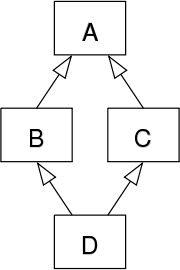
\includegraphics[height=0.5\textheight]{./Diamond_inheritance.png}
   \end{figure}
\end{frame}

\begin{frame}[plain,fragile]{Problema del diamante}{
  Qu\'e pasa con el siguiente c\'odigo?
}
   \begin{lstlisting}[style=normal,firstnumber=1,linebackgroundcolor={%
           \btLstHLR<1>{11}%
   }]
class A {
  int getEntero();
};

class B: public A {};
class C: public A {};
class D: public B, public C {};

int main(void) {
  D d;
  d.getEntero();
  return 0;
}

   \end{lstlisting}

   La l\'inea 11 no compila porque tanto B como C tienen su copia interna de los miembros de A, y por ende la llamada a \textbf{getEntero()} es ambigua.
\end{frame}

\begin{frame}[plain,fragile]{Problema del diamante - Soluci\'on}{
  Hacer que B y C hereden virtualmente de A. 
}
   \begin{lstlisting}[style=normal,firstnumber=1,linebackgroundcolor={%
           \btLstHLB<1>{11}%
   }]
class A {
  int getEntero();
};

class B: virtual public A {};
class C: virtual public A {};
class D: public B, public C {};

int main(void) {
  D d;
  d.getEntero();
  return 0;
}

   \end{lstlisting}
   Ahora D tendr\'a una sola copia interna de A.
\end{frame}

\appendix
\section<presentation>*{\appendixname}
\subsection<presentation>*{Referencias}

\begin{frame}[allowframebreaks]
   \frametitle<presentation>{Referencias}

   \begin{thebibliography}{10}

         \beamertemplatebookbibitems
         % Start with overview books.

      \bibitem{Stroustrup}
         Bjarne Stroustrup.
         \newblock {\em The C++ Programming Language}.
         \newblock Addison Wesley, Fourth Edition.

   \end{thebibliography}
\end{frame}

\end{document}


